\section{Build}
This section outlines the different build steps required to produce the final
system image containing the Muen separation kernel and all subjects as defined
by the system policy. Figure \ref{fig:build-process} illustrates the build
process.

\begin{figure}[h]
	\centering
	\begin{tikzpicture}[minimum height=0.6cm]
	\node (src) [apribox]               {Source Format};
	\node (mrg) [bluebox, right=of src] {Merger};
	\node (exp) [bluebox, right=of mrg] {Expander};
	\node (fma) [apribox, right=of exp] {Format A};
	\node (alo) [bluebox, right=of fma] {Allocator};
	\node (fmb) [apribox, below=of alo] {Format B};
	\node (val) [bluebox, left=of fmb]  {Validator};
	\node (sge) [bluebox, left=of val]  {Structure Generators};

	\node (spk) [graybox, below=of sge] {Source Specs};
	\node (iob) [graybox, right=of spk] {I/O Bitmaps};
	\node (msc) [graybox, right=of iob, minimum width=1.5cm] {...};
	\node (pta) [graybox, left=of spk] {Page Tables};
	\node (zpa) [graybox, left=of pta] {Zero Page};

	\node (bin) [apribox, below=of spk] {Binaries};

	\node (has) [bluebox, below=of bin] {Hasher};

	\node (sin) [bluebox, below=of has] {Sinfo};

	\node (pak) [bluebox, below=of sin] {Packer};

	\node (img) [apribox, below=of pak] {System Image};

	\draw[arrow] (src) -- (mrg);
	\draw[arrow] (mrg) -- (exp);
	\draw[arrow] (exp) -- (fma);
	\draw[arrow] (fma) -- (alo);
	\draw[arrow] (alo) -- (fmb);
	\draw[arrow] (fmb) -- (val);
	\draw[arrow] (val) -- (sge);

	\draw[arrow] (sge) -- (spk);
	\draw[arrow] (sge) -- (iob);
	\draw[arrow] (sge) -- (msc);
	\draw[arrow] (sge) -- (pta);
	\draw[arrow] (sge) -- (zpa);

	\draw[arrow] (spk) -- (bin);

	\draw[arrow] (bin) -- (has);
	\draw[arrow] (has) -- (sin);
	\draw[arrow] (sin) -- (pak);

	\draw[arrow] (msc) -- (pak);
	\draw[arrow] (iob) -- (pak);
	\draw[arrow] (iob) -- (pak);
	\draw[arrow] (pta) -- (pak);
	\draw[arrow] (zpa) -- (pak);

	\draw[arrow] (pak) -- (img);
\end{tikzpicture}

	\caption{Build process}
	\label{fig:build-process}
\end{figure}

The first step is to build the tools. The \texttt{skconfig} helper tool can be
used, as described in section \ref{subsec:subject-binary-analysis}, to create
subject initial state and memory layout specifications in XML format from the
subject binary. The generated XML files are included in the system policy before
the policy compilation step.

To compile the system policy, the \texttt{skpolicy} tool is required. The
details about the policy compilation process is described in section
\ref{subsec:policy-compilation}.  The Muen kernel and all subjects require the
Ada ZFS runtime described in section \ref{sec:zfs-rts} to compile. Once the
policy has been compiled and the ZFS runtime has been built, the kernel and all
subjects are built.

The final step is to package all object binaries (i.e. the kernel and all
subjects) including all related files into a bootable OS image. This task is
handled by the \texttt{skpacker} tool described in section
\ref{subsec:image-packaging}.

\subsection{Policy compilation}\label{subsec:policy-compilation}
The \texttt{skpolicy} tool compiles the XML system policy outlined in section
\ref{sec:policy} to different output formats as shown in figure
\ref{fig:policy-compilation}.

\begin{figure}[h]
	\centering
	\begin{tikzpicture}
	\node (pol) [greenbox]                            {Policy};
	\node (skp) [apribox, below=of pol]               {skpolicy};
	\node (sou) [bluebox, below=of skp, xshift=1.5cm] {Source specs};
	\node (pag) [bluebox, left=of sou]                {Page tables};
	\node (iob) [bluebox, left=of pag]                {I/O bitmaps};
	\node (msr) [bluebox, right=of sou]               {MSR bitmaps};

	\draw[arrow] (pol) to (skp);
	\draw[arrow] (skp) to (sou);
	\draw[arrow] (skp) to (msr);
	\draw[arrow] (skp) to (pag);
	\draw[arrow] (skp) to (iob);
\end{tikzpicture}

	\caption{Policy compilation}
	\label{fig:policy-compilation}
\end{figure}

The generated subject page tables, I/O and MSR bitmaps are included in the final
system image by the \texttt{skpacker} utility explained in the following section
\ref{subsec:image-packaging}. These files are all in binary form and correspond
to the format mandated by the respective Intel SDM chapters \cite{IntelSDM}.
Page tables are generated for subjects as well as for the kernel itself.

The generated SPARK and Assembly source specifications are included in the
kernel directly. These specifications provide the kernel with the following
information:

\begin{itemize}
	\item \emph{IRQ routing specification}\\
		Used by the kernel to program the system's I/O APIC for interrupt
		routing.
	\item \emph{Kernel address constants}\\
		Define kernel stack, page table and per-CPU storage memory addresses.
	\item \emph{Scheduling plans for all CPU cores}\\
		The scheduling plans are indexed by the logical processor's APIC ID.
		Each kernel copies its associated scheduling plan to the per-CPU storage
		area on initialization.
	\item \emph{Subjects specification}\\
		Defines all subjects and their parameters, see policy section
		\ref{subsec:subjects}.
	\item \emph{Packer specification}\\
		Defines the configuration used for the \texttt{skpacker} tool outlined
		in the following section \ref{subsec:image-packaging}.
\end{itemize}

\subsection{Subject binary analysis}\label{subsec:subject-binary-analysis}
The \texttt{skconfig} tool uses the Binary File Descriptor (BFD\index{BFG})
library to analyze subject binaries and creates appropriate XML\index{XML}
policy specifications from it, see figure \ref{fig:object-analysis}. This is
useful to generate the initial state and the memory layout directly from a
native subject binary instead of writing it by hand. The tool extracts stack
address, entry point and memory layout from a subject binary.

\begin{figure}[h]
	\centering
	\begin{tikzpicture}
	\node (obj) [bluebox]                {Binary object};
	\node (skc) [apribox,  below=of obj] {skconfig};
	\node (xml) [greenbox, below=of skc] {XML specification};

	\draw[arrow] (obj) to (skc);
	\draw[arrow] (skc) to (xml);
\end{tikzpicture}

	\caption{From binary object to XML specification}
	\label{fig:object-analysis}
\end{figure}

The exctracted subject initial state and memory layout XML specifications can be
included in the system policy before compilation by the \texttt{skpolicy} tool.
The generated memory layout is only as permissive as required by the original
subject binary. For example, the memory region mapped for executable code
(the \texttt{.text} section) will be executable but non-writeable. This is in
contrast to just providing a big enough memory region with all permissions to
the subject with no exact mapping of binary sections to memory access
permissions (i.e. read, write, execute).

\subsection{Image packaging}\label{subsec:image-packaging}
The \texttt{skpacker} tool is responsible to assemble the final bootable system
image from the parts produced in the previous build steps. Figure
\ref{fig:image-packaging} illustrates the process. The tool includes the special
packer source specification created from the system policy. This specification
includes information about subject binaries and their physical address in the
final image.

\begin{figure}[h]
	\centering
	\begin{tikzpicture}
	\node (knl) [bluebox]                              {Kernel binary};
	\node (sub) [bluebox, left=of knl]                 {Subject binaries};
	\node (pag) [bluebox, left=of sub]                 {Page tables};
	\node (bit) [bluebox, right=of knl]                {Bitmaps};
	\node (skp) [apribox, below=of knl, xshift=-1.5cm] {skpacker};
	\node (spe) [bluebox, left=of skp]                 {Packer spec};
	\node (sys) [greenbox, below=of skp]               {System image};

	\draw[arrow] (pag) to (skp);
	\draw[arrow] (sub) to (skp);
	\draw[arrow] (knl) to (skp);
	\draw[arrow] (bit) to (skp);
	\draw[arrow] (skp) to (sys);
	\draw[arrow] (spe) to (skp);
\end{tikzpicture}

	\caption{System image packaging}
	\label{fig:image-packaging}
\end{figure}

The remaining configuration is extracted from the source specification provided
to the kernel. Listing \ref{lst:skpacker} shows the output of a
\texttt{skpacker} run with the example system described in section
\ref{sec:example-system}. The fist column in the output designate physical
addresses in memory. The second column specifies the type of the packaged file
at this specific memory location. The abbreviations have the following meaning:

\begin{itemize}
	\item \emph{PML4} The file at this address designates a page table
		structure. It is either a page table for a kernel or for a subject. The
		kernels running on the different logical processors have different page
		tables to allow distinct stack and per-CPU storage pages transparently.
	\item \emph{IOBM} The file is a subject I/O bitmap. Specifies which I/O
		ports a subject is allowed to access.
	\item \emph{MSBM} The file is a subject MSR bitmap. Specifies which MSRs a
		subject is allowed to access.
	\item \emph{BIN} The file is a subject (raw) binary.
\end{itemize}

\begin{lstlisting}[
	caption=Example output of skpacker tool,
	label=lst:skpacker,
	frame=none,
	numbers=none]
         Packaging kernel image 'obj/kernel'
         0000000000200000 [PML4] kernel (0)
         0000000000204000 [PML4] kernel (1)
         0000000000208000 [PML4] kernel (2)
         000000000020c000 [PML4] kernel (3)
         0000000000210000 [PML4] tau0
         0000000000214000 [IOBM] tau0
         0000000000216000 [MSBM] tau0
         0000000000217000 [BIN ] tau0
         0000000000240000 [PML4] vt
         0000000000244000 [IOBM] vt
         0000000000246000 [MSBM] vt
         0000000000247000 [BIN ] vt
         0000000000270000 [PML4] crypter
         0000000000274000 [IOBM] crypter
         0000000000276000 [MSBM] crypter
         0000000000277000 [BIN ] crypter
         00000000002a0000 [PML4] sm
         00000000002a4000 [IOBM] sm
         00000000002a6000 [MSBM] sm
         00000000002a7000 [BIN ] sm
         00000000002d0000 [PML4] xv6 (EPT)
         00000000002d4000 [IOBM] xv6
         00000000002d6000 [MSBM] xv6
         00000000002d7000 [BIN ] xv6
\end{lstlisting}

Once the packaging step is complete, the resulting OS image can be booted by any
Multiboot \cite{multiboot} compliant bootloader.

\subsection{Emulation}
To ease kernel development, the Muen project makes heavy use of emulation using
the Bochs IA-32 emulator. Bochs has support for multiple processors, APIC
emulation and VMX extensions among others. This allows to run the Muen example
system described in the following section \ref{sec:example-system} as
illustrated by figure \ref{fig:bochs}.

\begin{figure}[h]
	\centering
	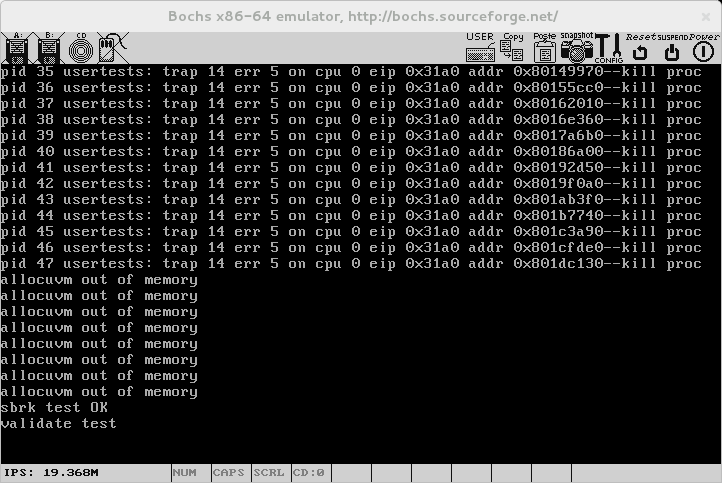
\includegraphics[width=\textwidth]{images/bochs}
	\caption{Bochs running the Muen example system}
	\label{fig:bochs}
\end{figure}

Bochs writes detailed logs during emulation and also provides a debugger which
allows to inspect the complete system state at any time. It has proven very
helpful when implementing new low-level processor features.
